\chapter{Effekte}
F"uer die veschiedenen F"ahigkeiten sowie schie"sen wurden Partikeleffekte erstellt.
Dazu wurde das Partikelsystem von Unity genutzt.

\begin{figure}
	\centering
	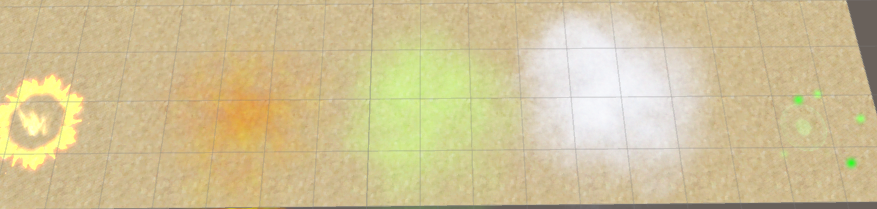
\includegraphics[height=4cm]{images/Partikeleffekte.png}
	\caption{Von Links nach Rechts: Explosion, Feuer, Gas, Rauch, Heileffekt}
	\label{fig:Effekte}
\end{figure}
